\documentclass{beamer}
\usepackage[latin1]{inputenc}
\usepackage[absolute,overlay]{textpos}
\usepackage{listings}
%\usetheme{Montpellier}
%\usetheme{Singapore}

%\usetheme{Warsaw}
%\useoutertheme{infolines}


%\usecolortheme[RGB={204,51,255}]{structure}
%\usecolortheme[named=purple]{structure}
\usecolortheme[RGB={62,128,62}]{structure}
%\definecolor{dark}{rgb}{0.3,0.15,0.3}
%\definecolor{light}{rgb}{0.8,0.6,0.8}
%\definecolor{reddish}{rgb}{.5,0.15,0.15}
\definecolor{dark}{rgb}{0.7,0.25,0.25}
%\definecolor{light}{rgb}{0.8,0.6,0.8}
\definecolor{reddish}{rgb}{.7,0.25,0.25}
\usepackage{graphicx}
\usepackage{pstricks}

\setbeamertemplate{navigation symbols}{}

\newcommand\FrameText[1]{%
  \begin{textblock*}{\paperwidth}(0pt,\textheight)
    \raggedright #1\hspace{.5em}
  \end{textblock*}}

\newcommand{\crish}{\color{reddish}}
\newcommand{\cbla}{\color{black}}
\newcommand{\cred}{\color{red}}
\newcommand{\cblu}{\color{blue}}
\newcommand{\cgre}{\color{green}}
\newcommand{\cpur}{\color{orange}}

\newcommand{\sm}{\color{reddish}$}
\newcommand{\fm}{$\color{black}{}}

\newcommand{\letter}[1]{\color{blue}\texttt{#1}\color{black}}
\newcommand{\binary}[1]{\color{red}\texttt{#1}\color{black}}



\lstset{
basicstyle=\ttfamily, 
columns=fullflexible, % make sure to use fixed-width font, CM typewriter is NOT fixed width
numbers=left, 
numberstyle=\small\ttfamily\color{gray},
stepnumber=1,              
numbersep=10pt, 
numberfirstline=true, 
numberblanklines=true, 
tabsize=4,
lineskip=-1.5pt,
extendedchars=true,
breaklines=true,        
keywordstyle=\color{blue}\bfseries,
identifierstyle=, % using emph or index keywords
commentstyle=\sffamily\color{OliveGreen},
stringstyle=\color{Maroon},
showstringspaces=false,
showtabs=false,
upquote=false,
texcl=true % interpet comments as LaTeX
}

\lstdefinelanguage{julia}
{
  keywordsprefix=\@,
  morekeywords={
    exit,whos,edit,load,is,isa,isequal,typeof,tuple,ntuple,uid,hash,finalizer,convert,promote,
    subtype,typemin,typemax,realmin,realmax,sizeof,eps,promote_type,method_exists,applicable,
    invoke,dlopen,dlsym,system,error,throw,assert,new,Inf,Nan,pi,im,begin,while,for,in,return,
    break,continue,macro,quote,let,if,elseif,else,try,catch,end,bitstype,ccall,do,using,module,
    import,export,importall,baremodule,immutable,local,global,const,Bool,Int,Int8,Int16,Int32,
    Int64,Uint,Uint8,Uint16,Uint32,Uint64,Float32,Float64,Complex64,Complex128,Any,Nothing,None,
    function,type,typealias,abstract
  },
  sensitive=true,
  morecomment=[l]{\#},
  morestring=[b]',
  morestring=[b]" 
}

\lstset{
    literate={~} {$\sim$\,\,}{1}
}

\usepackage{tikz}
\usetikzlibrary{arrows,decorations.markings,positioning}
\usepackage{epstopdf}
\usetikzlibrary{fit}

\title[Transfer entropy for population data.]{Transfer entropy for population data.}
\author{Conor Houghton}
\institute{U Bristol}
\date{Edinburgh, June 2022}

\begin{document}

\maketitle

\begin{frame}{Bayes rule}
  \crish
  $$p_{X,Y}(x,y)=p_{X|Y}(x|y)p_Y(Y)$$
  \cbla
  and
  \crish
  $$p_{X,Y}(x,y)=p_{Y|X}(y|x)p_X(x)$$
  \cbla
  so
  \crish
  $$p_{X|Y}(x|y)=\frac{p_{Y|X}(y|x)p_X(x)}{p_Y(y)}$$
  \cbla
  \end{frame}

\begin{frame}{Bayesian inference}
  \begin{quote}Bayesian inference applies Bayes rule to a \textbf{model}\end{quote}
  \begin{itemize}
  \item We have a \textbf{model} parameterized with some \textbf{parameters} \sm \theta\fm{}.
  \item We have some \textbf{data}.
  \end{itemize}
  \begin{quote} Bayesian inference tells us what we know about the parameters given the data.\end{quote}
\end{frame}



\begin{frame}{What does probability model?}
  \begin{quote}
    The laws of probability are mathematics - the mathematics don't determine what probabilities model.
  \end{quote}
    \begin{quote}
    In Bayesian inference probabilities describe our knowledge.
  \end{quote}
\end{frame}

\begin{frame}{Frequentists versus Bayesians}
  \begin{center}
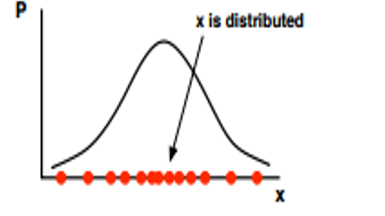
\includegraphics[width=4.125cm]{fig_freq.png}
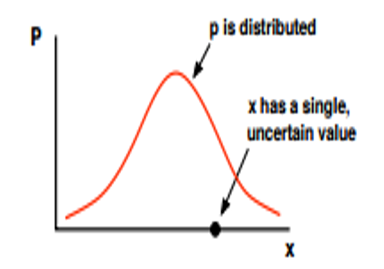
\includegraphics[width=3.75cm]{fig_bayes.png}
\end{center}
  \FrameText{\tiny{Picture from Rosalyn Moran}}  
\end{frame}

\begin{frame}{Guess the missing letter}
  \begin{tabular}{lc}
    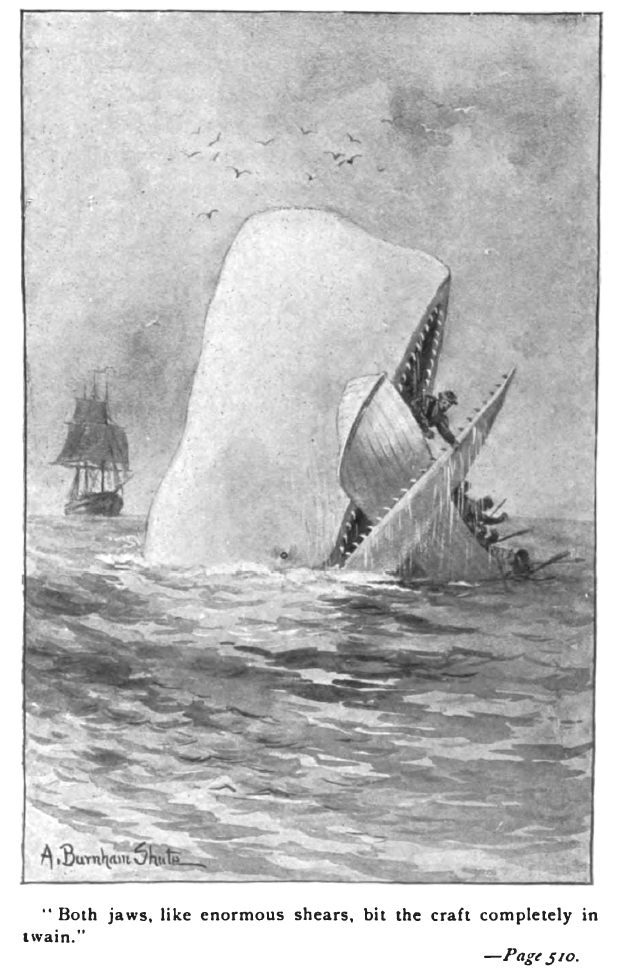
\includegraphics[width=4cm]{Moby_Dick.jpg}&\cred{}CALL ME ISHMAE*\cbla{}
  \end{tabular}
  \end{frame}


\begin{frame}{Guess the missing letter - letter frequencies}
  \begin{center}
    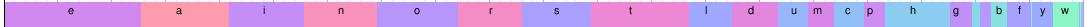
\includegraphics[width=11cm]{freq.png}
  \vskip 1cm
    \cred{}CALL ME ISHMAE\cblu{}*\cbla{}
  \end{center}
  with for example \crish$p(E)=0.13$\cbla{}, \crish$p(L)=0.04$\cbla{} and \crish$p(Q)=0.001$\cbla{}. 
  \FrameText{\tiny{Letter frequency table from Wikipedia}}  
  \end{frame}


\begin{frame}{Guess the missing letter - 2-gram letter frequencies}
  Look at two letter pairs, \textsl{ER} and \textsl{EL} and so on, and
  work out conditional probabilities like \crish$$ p(\mbox{second
    letter is L}|\mbox{first letter is E})
  $$\cbla{}
  \begin{center}
    \cred{}CALL ME ISHMA\cblu{}E*\cbla{}
  \end{center}
  with for example \crish$p(R)=0.14$\cbla{}, \crish$p(L)=0.04$\cbla{} and \crish$p(Q)=0.003$\cbla{}. 
  \end{frame}


\begin{frame}{Guess the missing letter - 3-gram letter frequencies}


    \begin{center}
    \cred{}CALL ME ISHM\cblu{}AE*\cbla{}
  \end{center}
  with for example \crish$p(R)=0.1$\cbla{}, \crish$p(L)=0.4$\cbla{} and \crish$p(P)=0.001$\cbla{}. 
  \end{frame}


\begin{frame}{Guess the missing letter}
  \begin{tabular}{lc}
    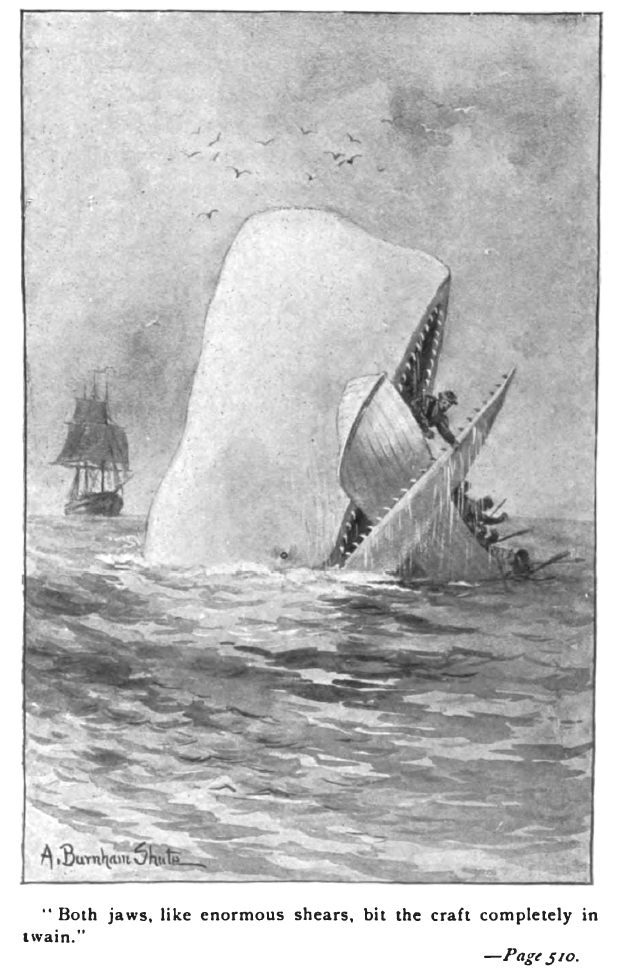
\includegraphics[width=4cm]{Moby_Dick.jpg}&\cred{}CALL ME ISHMAEL\cbla{}
  \end{tabular}
  \end{frame}

\begin{frame}{Bayesian inference}

  We have a \cblu\textbf{model}\cbla{} parameterized with some \cblu\textbf{parameters}\cbla{} say \sm \cblu\theta\crish\fm{}\cbla.\vskip 0.75cm
  We have \textbf{priors}, some knowledge of \sm \cblu\theta\fm{} described using probability distributions: \sm p(\cblu\theta\crish)\fm{}.\vskip 0.75cm
 We have some \cpur\textbf{data}\cbla{} points \cpur\sm\cpur\mathbf{x}_i\fm{}\color{black}.\vskip 0.75cm
We can calculate \sm p(\cpur\text{data}\crish|\cblu\text{model}\crish)\fm{}, that is \sm p(\cpur\textbf{x}_i\crish|\cblu\theta\crish)\fm{}.
  \vskip 1.5cm
  Bayesian inference is about calculating \sm{}p(\cblu\text{model}\crish|\cpur\text{data}\crish)\fm{}{} or \sm p(\cblu\theta\crish|\cpur\textbf{x}_i\crish)\fm{} using Bayes rule.
\end{frame}

\begin{frame}{Bayesian inference}

  \crish
  $$p(\cblu\text{model}\crish|\cpur\text{data}\crish)=\frac{p(\cpur\text{data}\crish|\cblu\text{model}\crish)p(\cblu\text{model}\crish)}{p(\cpur\text{data}\crish)}
    $$
    \cbla
    or
    \crish
    $$
p(\cblu\theta\crish|\cpur\textbf{x}_i\crish)=\frac{p(\cpur\textbf{x}_i\crish|\cblu\theta\crish)p(\cblu\theta\crish)}{p(\cpur\textbf{x}_i\crish)}
$$\cbla{}
\end{frame}

\begin{frame}{Example: interspike intervals}
  \begin{center}
    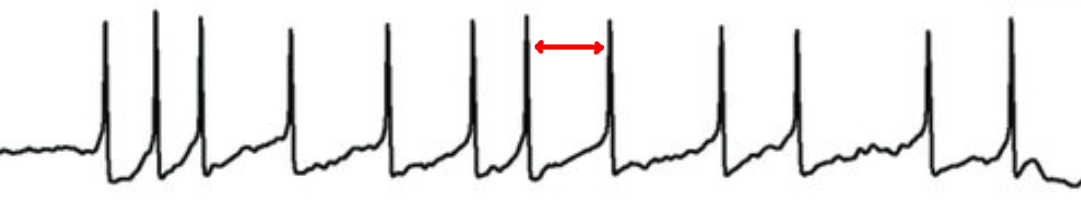
\includegraphics[width=10cm]{isi.png}
  \end{center}
\end{frame}

\begin{frame}{Interspike intervals: model}
    \begin{center}
    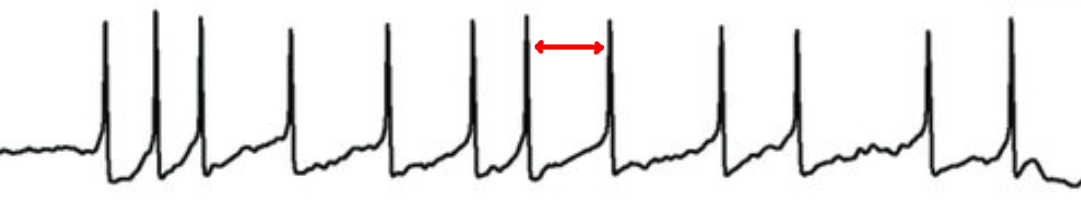
\includegraphics[width=7.5cm]{isi.png}
    \end{center}
    \cblu
    $$
    t\sim \text{Gamma}(k,\lambda)
    $$
    \cbla{}where \cblu$\lambda$\cbla{} is a scale parameter and \cblu$k$\cbla{} is a shape parameter: \cblu$\theta=(\lambda,k)$\cbla.
    \begin{center}
    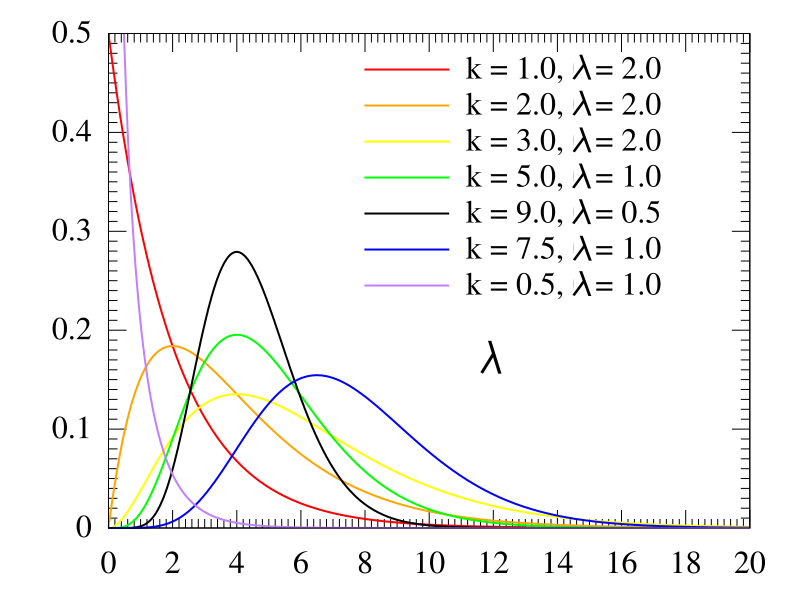
\includegraphics[width=6cm]{gamma.png}
    \end{center}
    \end{frame}
  

\begin{frame}{Interspike intervals: data}

For this example we will use the a spike train recorded from blowfly
viewing a visual stimulus:\vskip 1cm
\texttt{www.gatsby.ucl.ac.uk/~dayan/book/exercises.html}


\end{frame}

\begin{frame}{Interspike intervals: priors}

  Working out the mean and variance gives us some idea what the priors should be!
  \crish
  $$\mu=k\lambda$$
  \cbla{}and\crish
  $$\sigma^2=k\lambda^2$$
  \cbla{}so, this gives us\cblu
  $$\lambda\approx 0.027\text{ s}$$
  \cbla{}and \cblu
  $$k\approx 0.30$$
  \cbla
  We also know these parameters need to be positive so we will an exponential distribution.
  
\end{frame}

\begin{frame}{Model and priors}
  Priors\cblu{}
  \begin{eqnarray*}
    \lambda&\sim&\text{Exp}(0.027)\cr
    k&\sim& \text{Exp}(0.3)\cr
  \end{eqnarray*}
  \cbla{}and data\crish
  $$\cpur{}t_i\crish\sim \text{Gamma}(\cblu{}k\crish,\cblu{}\lambda\crish)$$
  \cbla

\end{frame}


\begin{frame}{Posteriors}
\vskip 1cm
Now all we need to do is work out the \textsl{posterior}: \crish{}$p(\cblu{}\lambda\crish,\cblu{}k\crish|\cpur{}t_i\crish)$.
\vskip 1cm
In principle this is just Bayes rule
\crish
$$
p(\cblu\lambda\crish,\cblu{}k\crish|\cpur{}t_i\crish)=\frac{p(\cpur{}t_i\crish|\cblu\lambda\crish,\cblu{}k\crish)p(\cblu\lambda\crish,\cblu{}k\crish)}{p(\cpur{}h_i\crish)}
$$\cbla{}
However, in practice we can't usually can't do this calculation, calculating \crish$p(\cpur{}h_i\crish)$\cbla{} involves doing an integral we can't do!
\end{frame}

\begin{frame}{Posteriors}
  \vskip 1cm
We need to work out the \textsl{posterior}: \crish{}$p(\cblu{}\lambda\crish,\cblu{}k\crish|\cpur{}t_i\crish)$.\cbla{}
\vskip 1cm
In practice we calculate the posterior using \textbf{magic}. The name of this magic is the \textsl{No-U Turn Sampler} or \textsl{NUTS}.
\vskip 1cm NUTS is one of the things that makes Bayesian inference
possible and practical all of a sudden. It is important to understand
it and to develop a feel for when it will work well and when small
changes to an approach will make it work better. Here we will treat it
as \textbf{magic}.
\end{frame}

\begin{frame}{NUTS}
  \vskip 1cm
  A number of languages or libraries allow you to use NUTS;
  most obviously \texttt{STAN}, \texttt{turing.jl} and \texttt{PyMC3}.
  \vskip 1cm
  Here we will look at some \texttt{turing.jl} code as a sort of pseudocode
\end{frame}



\begin{frame}[fragile]{Some code}

\begin{lstlisting}[language=julia]
@model function gammaModel(isi)
       p=parameters(isi)
       meanL=p[1]
       meanK=p[2]  

       l ~ Exponential(meanL)
       k ~ Exponential(meanK) 

       for i in 1:length(isi)
       	   isi[i] ~ Gamma(k,l)
       end	   

end

chain = sample(gammaModel(isi), NUTS(), 1000)
\end{lstlisting}

\end{frame}

\begin{frame}{Results}
  \vskip 1cm
  Using 10 s of data; that is 1221 ISIs we get:
  \vskip 1cm
  \begin{center}
    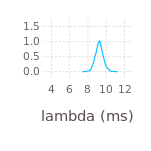
\includegraphics[width=4cm]{lambda10000.png}\qquad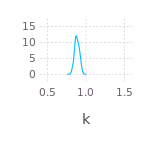
\includegraphics[width=4cm]{k10000.png}
  \end{center}
with \cblu$\bar{\lambda}=0.0093$\cbla{} and \cblu$\bar{k}=0.8861$\cbla.
\end{frame}


\begin{frame}{What?}
\vskip 1cm
\cblu$\bar{\lambda}=0.0093$\cbla{} and \cblu$\bar{k}=0.8861$\cbla.
\vskip 1cm
but didn't we say
\cblu
  $$\lambda\approx 0.027\text{ s}$$
  \cbla{}and \cblu
  $$k\approx 0.30$$
  \cbla
  before, by calculating the empirical mean and variance?
\end{frame}


\begin{frame}{Optimizing the log-pdf}
\vskip 1cm
\cblu$\bar{\lambda}=0.0093$\cbla{} and \cblu$\bar{k}=0.8861$\cbla.
\vskip 1cm
and by optimizing the log-pdf\crish
$$
L=\sum_i \log{p(\cpur\delta t_i\crish|\cblu{}\lambda\crish,\cblu{}k\crish)}$$
\cbla{}over $\cblu{}\lambda\crish,\cblu{}k\crish$.\cbla{} This gives
\cblu
  $$\lambda\approx 0.092\text{ s}$$
  \cbla{}and \cblu
  $$k\approx 0.89$$
  \cbla
  which gives a similar answer!
\end{frame}


\begin{frame}{Results - what does Bayes buy you?}
  \vskip 1cm
  Why not just optimize the log-pdf!
  \vskip 1cm
  With Bayes we know what we know!
  \end{frame}


\begin{frame}{Results - what does Bayes buy you?}
  \vskip 1cm
  Using 1 s of data; that is 146 ISIs we get:
  \vskip 1cm
  \begin{center}
    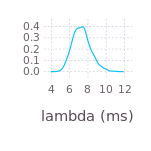
\includegraphics[width=4cm]{lambda1000.png}\qquad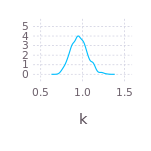
\includegraphics[width=4cm]{k1000.png}
  \end{center}
  \end{frame}


\end{document}

